\section{Post-Training}
\label{section:finetuning}
We produce the aligned \llamathree~models by applying several rounds of post-training,\footnote{We use the term ``post-training'' to refer to any model training that happens outside of pre-training.} or aligning the model with human feedback~\citep{ouyang2022instructgpt,rafailov2024direct} on top of a pre-trained checkpoint. Each round of post-training involves supervised finetuning (SFT) followed by Direct Preference Optimization~\citep[DPO;][]{rafailov2024direct} on examples collected either via human annotations or generated synthetically. Our post-training modeling and data approaches are described in Sections~\ref{sec:finetuning_modeling} and ~\ref{sec:finetuning_data} respectively.
We further detail custom data curation strategies to improve the reasoning, coding, factuality, multilingual, tool use, long context, and precise instruction following in Section~\ref{sec:Capabilities}.

\begin{figure}[t]
    \centering
    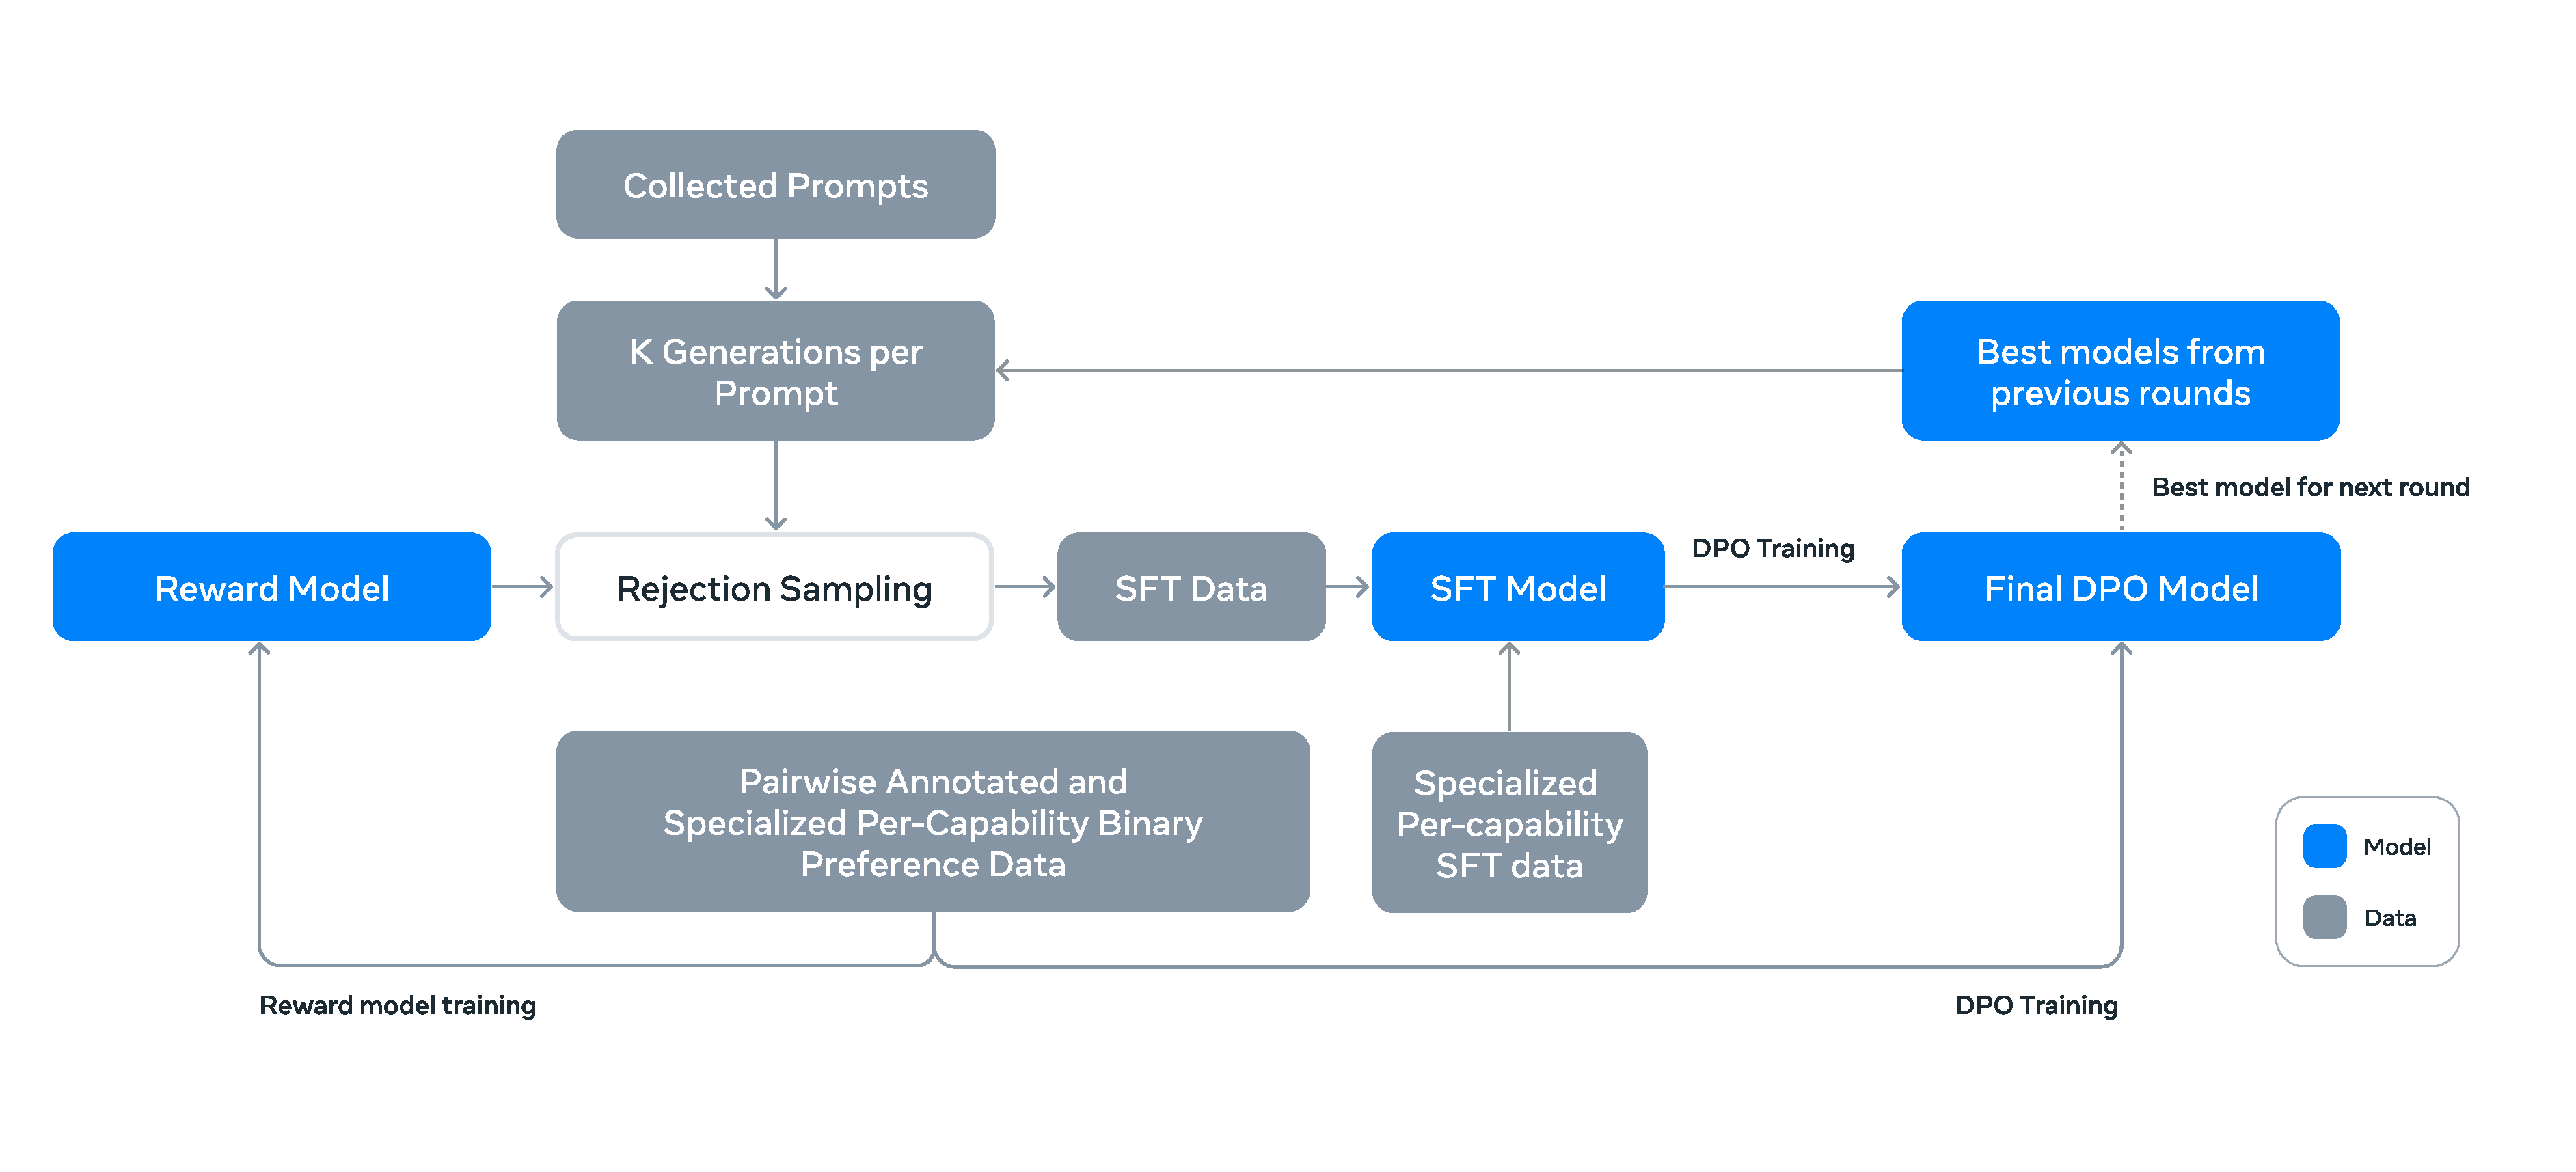
\includegraphics[width=\textwidth]{assets/posttraining_overview.pdf}
    \caption{\textbf{Illustration of the overall post-training approach for Llama 3.} Our post-training strategy involves rejection sampling, supervised finetuning, and direct preference optimization. See text for details.}
    \label{fig:posttraining_overview}
\end{figure}

\subsection{Modeling}
\label{sec:finetuning_modeling}
The backbone of our post-training strategy is a reward model and a language model. We first train a reward model on top of the pre-trained checkpoint using human-annotated preference data (see Section~\ref{subsubsec:rm}). We then finetune pre-trained checkpoints with supervised finetuning (SFT; see Section~\ref{subsubsec:sft}), and further align the checkpoints with Direct Preference Optimization (DPO; see Section~\ref{subsubsec:postdpo}).
This process is illustrated in Figure~\ref{fig:posttraining_overview}.
Unless otherwise noted, our modeling procedure applies to \llamathree~405B, and we refer to \llamathree~405B as \llamathree~for simplicity. 

\subsubsection{Chat Dialog Format}
\label{subsubsec:chat_format_content}

To tune LLMs for human-AI interaction, we need to define a chat dialog protocol for the model to understand human instructions and perform conversational tasks. Compared to its predecessor, \llamathree~has new capabilities such as tool use (Section~\ref{subsubsec:tool_use}) which may require generating multiple messages and sending them to different locations (e.g., user, \texttt{ipython}) within a single dialog turn. To support this, we design a new multi-message chat protocol which uses various special header and termination tokens. The header tokens are used to indicate the source and destination of each message in a conversation. Similarly, the termination tokens indicate when it is the time to alternate between human and AI to speak. 

\subsubsection{Reward Modeling}
\label{subsubsec:rm}

We train a reward model (RM) covering different capabilities on top of the pre-trained checkpoint. The training objective is the same as \llamatwo~except that we remove the margin term in the loss, as we observe diminishing improvements after data scaling. Following Llama 2, we use all of our preference data for reward modeling after filtering out samples with similar responses. In addition to standard preference pair of (chosen, rejected) response, annotations also create a third ``edited response'' for some prompts, where the chosen response from the pair is further edited for improvement (see Section~\ref{sec:rlhf_annotation_data}). Hence, each preference ranking sample has two or three responses with clear ranking (\emph{edited} > \emph{chosen} > \emph{rejected}). We concatenate the prompt and multiple responses into a single row during training with responses randomly shuffled. This is an approximation to the standard scenario of putting the responses in separate rows and computing the scores, but in our ablations, this approach improves training efficiency without a loss in accuracy. 


\subsubsection{Supervised Finetuning}
\label{subsubsec:sft}
The reward model is then used to perform rejection sampling on our human annotation prompts, the details of which are described in Section~\ref{sec:finetuning_data}. Together with this rejection-sampled data and other data sources (including synthetic data), we finetune the pre-trained language model using a standard cross entropy loss on the target tokens (while masking loss on prompt tokens).
More details about the data mix can be found in Section~\ref{sec:finetuning_data}.
We refer to this stage as \emph{supervised finetuning} \citep[SFT;][]{weifinetuned,sanh2022multitask,wang2022super}, even though many of the training targets are model-generated.
Our largest models are finetuned with a learning rate of $10^{-5}$ over the course of 8.5K to 9K steps. We found these hyperparameter settings to work well across different rounds and data mixes.

\subsubsection{Direct Preference Optimization}
\label{subsubsec:postdpo}

We further train our SFT models with Direct Preference Optimization \citep[DPO;][]{rafailov2024direct} for human preference alignment. For training, we primarily use the most recent batches of preference data collected using the best performing models from the previous alignment rounds. As a result, our training data conforms better to the distribution of the policy model that is being optimized in each round. We also explored on-policy algorithms such as PPO~\citep{schulman2017proximal}, but found that DPO required less compute for large-scale models and performed better, especially on instruction following benchmarks like IFEval~\citep{zhou2023instruction}.
For Llama~3, we use a learning rate of $10^{-5}$ and set the $\beta$ hyper-parameter to be 0.1. In addition, we apply the following algorithmic modifications to DPO:

\begin{itemize}
    \item \textbf{Masking out formatting tokens in DPO loss}: We mask out special formatting tokens including header and termination tokens (described in Section~\ref{subsubsec:chat_format_content}) from both chosen and rejected responses in the loss to stabilize DPO training. We observe that having these tokens contribute to the loss may lead to undesired model behaviors such as tail repetition or abruptly generating termination tokens. We hypothesize that this is due to the contrastive nature of the DPO loss -- the presence of common tokens in both chosen and rejected responses leads to a conflicting learning objective as the model needs to increase and reduce the likelihood of these tokens simultaneously. 
    \item \textbf{Regularization with NLL loss}: We add an additional negative log-likelihood (NLL)  loss term with a scaling coefficient of $0.2$ on the chosen sequences, similar to~\citet{pang2024iterative}. This helps further stabilize DPO training by maintaining desired formatting for generation and preventing the decrease of log probability of chosen responses~\citep{pang2024iterative, pal2024smaug}. 
\end{itemize}

\subsubsection{Model Averaging}

Finally, we average models obtained from experiments using various versions of data or hyperparameters at each RM, SFT, or DPO stage~\citep{izmailov2019averagingweightsleadswider,wortsman2022modelsoupsaveragingweights, li2022branchtrainmergeembarrassinglyparalleltraining}. 

\subsubsection{Iterative Rounds}

Following Llama 2, we apply the above methods in six rounds. In each cycle, we collect new preference annotations and SFT data, sampling synthetic data from the latest models. 

\subsection{Post-training Data}
\label{sec:finetuning_data}

The post-training data composition plays a critical role in the usefulness and behavior of language models. In this section, we discuss our human annotation procedures and preference data collection (Section~\ref{sec:rlhf_annotation_data}), the composition of our SFT data (Section~\ref{subsubsec:sft_data}), and methods for data quality control and cleaning (Section~\ref{subsubsec:data_clean}).


\subsubsection{Preference Data} 
\label{sec:rlhf_annotation_data}

Our preference data annotation process is similar to Llama~2. We deploy multiple models for annotation after each round and sample two responses from two different models for each user prompt. These models can be trained with different data mixes and alignment recipes, allowing for different capability strength (\emph{e.g.}, code expertise) and increased data diversity. We ask annotators to rate the strength of their preference by categorizing it into one of four levels, based on how much more they prefer the chosen response over the rejected one: significantly better, better, slightly better, or marginally better. We also incorporate an editing step after preference ranking to encourage annotators to further improve the preferred response. Annotators edit the chosen response directly or prompt the model with feedback to refine its own response. Consequently, a portion of our preference data has three responses ranked (\emph{edited} > \emph{chosen} > \emph{rejected}).

In Table~\ref{tab:pref_data}, we report the statistics of preference annotations that we use for \llamathree training. 
General English covers multiple subcategories such as knowledge-based question and answering or precise instruction-following, which fall outside the scope of specific capabilities. Compared to Llama~2, we observe an increase in the average length of prompt and response, suggesting that we train \llamathree on more complex tasks. In addition, we implement a quality analysis and human evaluation process to rigorously assess the data collected, allowing us to refine our prompts and provide systematic, actionable feedback to annotators. For example, as \llamathree improves after each round, we increase prompt complexity accordingly to target areas where the model lags.

In each round of post-training, we use all the preference data that is available at the time for reward modeling, while only using the latest batches from various capabilities for DPO training. For both reward modeling and DPO, we use samples that are labeled as the chosen response being significantly better or better than the rejected counterpart for training and discard samples with similar responses.

\begin{table}[t]
  \centering
  \setlength{\tabcolsep}{4pt}
   {
  \begin{tabular}{@{}l@{\hspace*{0mm}}rrrrr@{}}
    \toprule
      & \textbf{\% of} & \textbf{Avg. \# turns} & \textbf{Avg. \# tokens} & \textbf{Avg. \# tokens} & \textbf{Avg. \# tokens} \\
     \textbf{Dataset} & \textbf{comparisons} &\textbf{per dialog} & \textbf{per example} &\textbf{in prompt} & \textbf{in response} \\
    \midrule
    General English & 81.99\% & 4.1 & 1,000.4 & 36.4 & 271.2 \\
    Coding & 6.93\% & 3.2 & 1,621.0 & 113.8 & 462.9 \\
    Multilingual & 5.19\% & 1.8 & 1,299.4 & 77.1 & 420.9 \\ 
    Reasoning and tools & 5.89\% & 1.6 & 707.7 & 46.6 & 129.9 \\
    \midrule
    Total & 100\% & 3.8 & 1,041.6 & 44.5 & 284.0 \\
    \bottomrule
  \end{tabular}}
  \vspace{0.3cm}
  \caption{\textbf{Statistics of human preference data.} We list statistics of the internally collected human preference data used for \llamathree alignment. We ask annotators to perform multi-turn dialogues with the models and make comparisons among responses at each turn. In post-processing, we split each dialogue to multiple examples at a turn level. Each example consists of a prompt (including previous dialog if available) and a response (e.g., chosen or rejected response).}
  \label{tab:pref_data}
\end{table}



\subsubsection{SFT Data}
\label{subsubsec:sft_data} 

Our finetuning data is largely comprised of the following sources:

\begin{itemize}
    \item Prompts from our human annotation collection with rejection-sampled responses.
    \item Synthetic data targeting specific capabilities (see Section~\ref{sec:Capabilities} for more details).
    \item Small amounts of human-curated data (see Section~\ref{sec:Capabilities} for more details).
\end{itemize}

As our post-training rounds progress, we develop stronger \llamathree variants that we use to collect larger datasets that cover a wide range of complex capabilities. In this section, we discuss the details for the rejection-sampling procedure and overall composition of our final SFT datamix.


\textbf{Rejection sampling.}
During rejection sampling (RS), for each prompt collected during human annotation (Section~\ref{sec:rlhf_annotation_data}) we sample $K$ (typically between 10 and 30) outputs from the latest chat model policy (usually the best performing checkpoint from the previous post-training iteration, or the best performing checkpoint for a particular capability) and use our reward model to select the best candidate, consistent with~\citet{constitutional-ai-bai}. 
In later rounds of post-training, we introduce system prompts to steer RS responses to conform with desirable tone, style, or formatting, which might be different for different capabilities. 

To increase the efficiency of rejection sampling, we adopt PagedAttention~\citep{kwon2023efficient}.
PagedAttention enhances memory efficiency through dynamic key-value cache allocation. 
It supports arbitrary output lengths by dynamically scheduling requests based on the current cache capacity.
Unfortunately, this carries the risk of swap-out when running out of memory. 
To eliminate such swap overhead, we define a maximum output length and perform a request only if sufficient memory is available to fit an output with that length.
PagedAttention also enables us to share the key-value cache pages for a prompt across all corresponding outputs.
Together, this leads to a throughput improvement of over $2 \times$ during rejection sampling.


\textbf{Overall data composition.} Table~\ref{tab:sft_data} shows data statistics for each broad category of our ``helpfulness'' mix. 
While SFT and preference data contain overlapping domains, they are curated differently, yielding distinct count statistics. In Section~\ref{subsubsec:data_clean} we describe techniques for categorizing topic, complexity, and quality of our data samples. In each round of post-training, we adjust our overall data mix carefully across these axes to tune performance across a wide range of benchmarks. Our final data mix epochs multiple times on some high quality sources and downsamples others.


\begin{table}[t]
  \centering
  \setlength{\tabcolsep}{4pt}
   {
  \begin{tabular}{@{}l@{\hspace*{0mm}}rrrrr@{}}
    \toprule
      & & & & \textbf{Avg. \# tokens} & \textbf{Avg. \# tokens} \\
     \textbf{Dataset} & \textbf{\% of examples} & \textbf{Avg. \# turns} & \textbf{Avg. \# tokens} & \textbf{in context} & \textbf{in final response} \\
   \midrule
   General English & 52.66\% & 6.3 & 974.0 & 656.7 & 317.1\\
    Code & 14.89\% & 2.7 & 753.3 &  378.8  & 374.5 \\
    Multilingual & 3.01\% & 2.7 & 520.5 & 230.8 & 289.7 \\
    Exam-like & 8.14\% & 2.3 & 297.8 &  124.4 & 173.4 \\
    Reasoning and tools & 21.19\% & 3.1  & 661.6 & 359.8 & 301.9 \\
    Long context & 0.11\% & 6.7 & 38,135.6 & 37,395.2 & 740.5 \\
    \midrule
    Total & $100\%$ & 4.7 & 846.1 & 535.7 & 310.4 \\
    \bottomrule
  \end{tabular}}
  \vspace{0.3cm}
  \caption{\textbf{Statistics of SFT data.} We list internally collected SFT data used for \llamathree alignment. Each SFT example consists of a context (i.e., all conversation turns except the last one) and a final response.}
  \label{tab:sft_data}
\end{table}



\subsubsection{Data Processing and Quality Control}
\label{subsubsec:data_clean} 

Given that most of our training data is \emph{model-generated}, it requires careful cleaning and quality control. 

\textbf{Data cleaning.} In the early rounds, we observed a number of undesirable patterns common in our data, such as excessive use of emojis or exclamation points. Therefore, we implement a series of rule-based data removal and modification strategies to filter or clean problematic data. For example, to mitigate overly-apologetic tonal issues, we identify overused phrases (such as ``I'm sorry'' or ``I apologize'') and carefully balance the proportion of such samples in our dataset. 


\textbf{Data pruning.} 
We also apply a collection of model-based techniques to remove low-quality training samples and improve overall model performance:

\begin{itemize}
    \item \textbf{Topic classification:} We first finetune \llamathree 8B into a topic classifier, and perform inference over all data to classify it into both coarsely-grained buckets (``mathematical reasoning'') and fine-grained buckets (``geometry and trigonometry''). 

    \item \textbf{Quality scoring:} We use both reward model and Llama-based signals to obtain a quality score for each sample. 
    For an RM-based score, we consider data that is in the top quartile of RM scores as high quality.
    For a Llama-based score, we prompt \llamathree~checkpoint to rate each sample on a three-point scale for general English data (accuracy, instruction following, and tone/presentation) and a two-point scale for coding data (bug identification and user intention), and consider samples that obtain the maximum score as high quality. 
    The RM and Llama-based scores have high disagreement rates, and we find that combining these signals yield the best recall on our internal test set. Ultimately, we select examples that are marked as high quality by the RM \emph{or} the Llama-based filter. 

    \item \textbf{Difficulty scoring:} 
    Because we are also interested in prioritizing examples that are more complex for the model, we score data using two measures of difficulty: Instag \citep{lu2023instag} and Llama-based scoring. For Instag, we prompt \llamathree 70B to perform intention tagging of SFT prompts, where more intentions implies more complexity. We also prompt \llamathree to measure the difficulty \citep{liu2024makesgooddataalignment} of dialogs on a three-point scale. 

    \item \textbf{Semantic deduplication:} Finally, we perform semantic deduplication \citep{abbas2023semdedup, liu2024makesgooddataalignment}. We first cluster complete dialogs using RoBERTa \citep{liu_ott_roberta} and within each cluster sort them by quality score $\times$ difficulty score. We then do greedy selection by iterating through all sorted examples, and only keeping the ones that have maximum cosine similarity less than a threshold to the examples seen so far in the cluster.

\end{itemize}


\subsection{Capabilities}
\label{sec:Capabilities}

We highlight special efforts to improve performance for specific capabilities such as code (Section~\ref{subsubsec:code}), multilinguality (Section~\ref{subsubsec:multilingual}), math and reasoning (Section~\ref{subsubsec:reasoning}), long context (Section~\ref{subsubsec:long_context}), tool use (Section~\ref{subsubsec:tool_use}), factuality (Section~\ref{subsubsec:factuality}), and steerability (Section~\ref{subsubsec:steerability}).  

\subsubsection{Code}
\label{subsubsec:code}

LLMs for code have received significant attention since the release of Copilot and Codex~\citep{chen2021evaluating}. 
Developers are now widely using these models to generate code snippets, debug, automate tasks, and improve code quality.
For \llamathree, we target improving and evaluating code generation, documentation, debugging, and review capabilities for the following high priority programming languages: Python, Java, Javascript, C/C++, Typescript, Rust, PHP, HTML/CSS, SQL, bash/shell. 
Here, we present our work on improving these coding capabilities via training a code expert, generating synthetic data for SFT, improving formatting with system prompt steering, and creating quality filters to remove bad samples from our training data.

\textbf{Expert training.} We train a \textbf{code expert} which we use to collect high quality human annotations for code throughout subsequent rounds of post-training. This is accomplished by branching the main pre-training run and continuing pre-training on a 1T token mix of mostly (>85\%) code data. Continued pre-training on domain-specific data has been shown to be effective for improving performance in a specific domain~\citep{gururangan2024dontstoppretraining}. We follow a recipe similar to that of CodeLlama \citep{codellama}. For the last several thousand steps of training we perform {long-context finetuning} (LCFT) to extend the expert's context length to 16K tokens on a high quality mix of repo-level code data. Finally, we follow the similar post-training modeling recipes described in Section~\ref{sec:finetuning_modeling} to align this model, except with SFT and DPO data mixes primarily targeting code.  This model is also used for rejection sampling (Section~\ref{subsubsec:sft_data}) for coding prompts.

\textbf{Synthetic data generation.}
During development, we identified key issues in code generation, including difficulty in following instructions, code syntax errors, incorrect code generation, and difficulty in fixing bugs. While intensive human annotation could theoretically resolve these issues, synthetic data generation offers a complementary approach at a lower cost and higher scale, unconstrained by the expertise level of annotators. As such, we use \llamathree and the code expert to generate a large quantity of synthetic SFT dialogs. 

We describe three high-level approaches for generating synthetic code data. In total, we generate over $2.7$M synthetic examples which were used during SFT.

\begin{enumerate}
    \item{\textbf{Synthetic data generation: execution feedback.}} The 8B and 70B models show significant performance improvements when trained on data generated by a larger, more competent model. However, our initial experiments revealed that training \llamathree 405B on its own generated data is not helpful (and can even degrade performance). To address this limitation, we introduced execution feedback as a source of truth, enabling the model to learn from its mistakes and stay on track. %
    In particular, we generate large dataset of approximately one million synthetic coding dialogues using the following process:


    \begin{itemize}
        \item \textbf{Problem description generation:}
        First, we generate a large collection of programming problem descriptions that span a diverse range of topics, including those in the long tail distribution. To achieve this diversity, we sample random code snippets from various sources and prompt the model to generate programming problems inspired by these examples. This allowed us to tap into a wide range of topics and create a comprehensive set of problem descriptions~\citep{wei2024magicoderempoweringcodegeneration}.
        
        
        \item \textbf{Solution generation:} Then, we prompt \llamathree to solve each problem in a given programming language. We observe that adding general rules of good programming to the prompt improves the generated solution quality. Also, we find it is helpful to require the model to explain its thought process in comments.
        
        \item \textbf{Correctness analysis:}
        After generating a solution, it is crucial to recognize that its correctness is not guaranteed, and including incorrect solutions in the finetuning dataset could harm the model's quality. While we do not ensure complete correctness, we develop methods to approximate it. To achieve this, we extract the source code from the generated solution and applied a combination of static and dynamic analysis techniques to test its correctness, including:
        
        \begin{itemize}{
        \item \textbf{Static analysis}: We run all generated code through a parser and a linter to ensure syntactic correctness, catching errors such as syntax errors, use of uninitialized variables or non-imported functions, code style issues, typing errors, and others.
        \item \textbf{Unit test generation and execution}: For each problem and solution, we prompt the model to generate unit tests, executed in a containerized environment together with the solution, catching run-time execution errors and some semantic errors.
        }\end{itemize}
        
        \item \textbf{Error feedback and iterative self-correction:}
        When a solution fails at any step, we prompt the model to revise it. The prompt included the original problem description, the faulty solution, and feedback from the parser/linter/tester (stdout, stderr/ and return code). %
        After a unit test execution failure, the model could either fix the code to pass the existing tests or modify its unit tests to accommodate the generated code.
        Only dialogs that pass all checks are included in the final dataset, used for supervised finetuning (SFT). Notably, we observed that about 20\% of solutions were initially incorrect but self-corrected, indicating that the model learned from the execution feedback and improved its performance.
        
        \item \textbf{Fine-tuning and iterative improvement:} The finetuning process is conducted over multiple rounds, with each round building on the previous one. After each round, the model is improved, generating higher-quality synthetic data for the next round. This iterative process allows for progressive refinement and enhancement of the model's performance.
    \end{itemize}

    \item{\textbf{Synthetic data generation: programming language translation.}} We observe a performance gap between major programming languages (\emph{e.g.}, Python/C++) and less common ones (\emph{e.g.}, Typescript/PHP). This is not surprising as we have less training data for less common programming languages. To mitigate this, we supplement our existing data by \emph{translating} data from common programming languages to less common languages (similar to \cite{chen2023breakinglanguagebarriersmultilingual} in the context of reasoning). This is achieved by prompting \llamathree and ensuring quality via syntax parsing, compilation, and execution. Figure~\ref{fig:code_translation_example} demonstrates an example of synthetic PHP code translated from Python. This improves performance significantly for less common languages as measured by the MultiPL-E \citep{cassano2022multiple} benchmark. 
    
    \begin{figure}
    \centering
    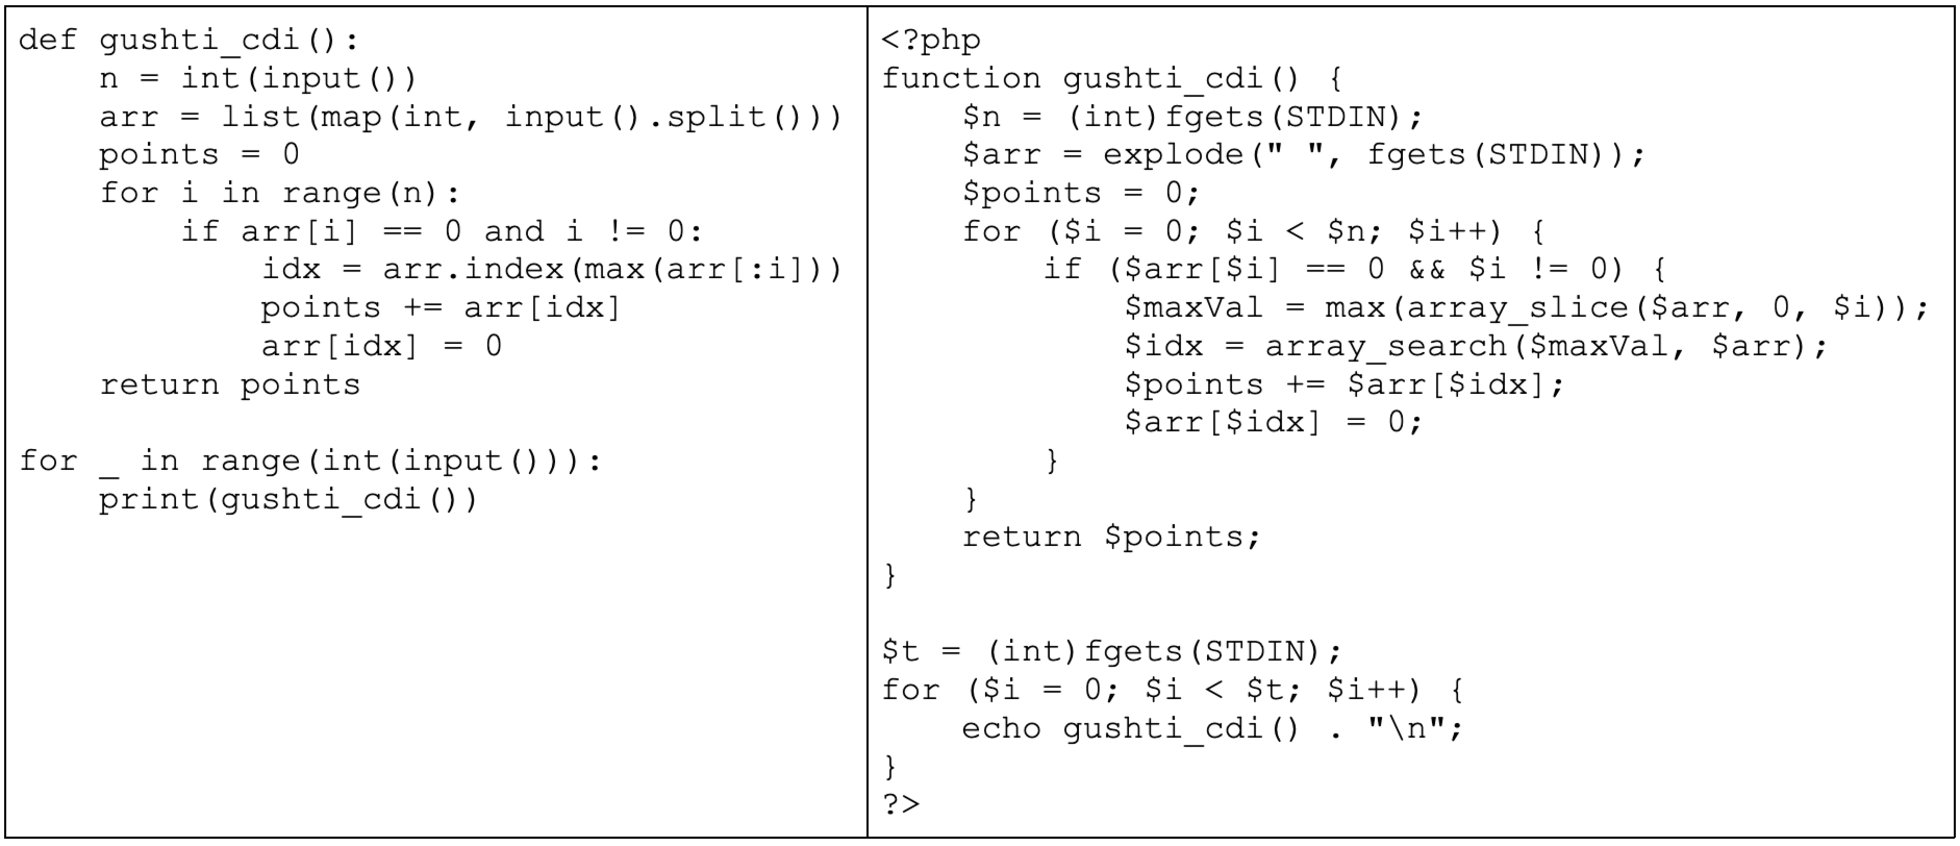
\includegraphics[width=0.75\linewidth]{posttraining/assets/code_translation_example.pdf}
    \caption{\label{fig:code_translation_example} \textbf{Code translation example.} We display an example of using \llamathree to translate Python code (left) to PHP code (right) to augment our SFT dataset with a wider range of programming languages.}
    \end{figure}


    \item{\textbf{Synthetic data generation: backtranslation.}} To improve certain coding capabilities (e.g., documentation, explanations) where execution feedback is less informative for determining quality, we employ an alternative multi-step approach. Using this procedure, we generated approximately 1.2M synthetic dialogs related to code explanation, generation, documentation, and debugging. Beginning with code snippets from a variety of languages in our pre-training data:
    \begin{itemize}
        \item \textbf{Generate:} We prompt \llamathree~to generate data that represents our target capability (e.g., we add comments and docstrings for the code snippet, or we ask the model to explain a piece of code).
        \item \textbf{Backtranslate:} We then prompt the model to ``backtranslate'' the synthetically generated data to the original code (e.g., we prompt the model to generate code only from its documentation, or we ask the model to generate code only from its explanation).
        \item \textbf{Filter:} Using the original code as a reference, we prompt the \llamathree to determine the quality of the output (e.g., we ask the model how faithful the backtranslated code is to the original). We then use the generated examples that have the highest self-verification scores in SFT. 
    \end{itemize}

\end{enumerate}


\textbf{System prompt steering during rejection sampling.} 
During the rejection sampling process, we used code specific system prompts to improve 
code readability, documentation, thoroughness, and specificity. Recall, from Section~\ref{tab:sft_data} this data is used to finetune the language model.  Figure \ref{fig:code_system_prompt_example} shows an example of how the system prompt helps improve the generated code quality --- it  adds necessary comments, uses more informative variable names, saves memory, etc.

\begin{figure}
\centering
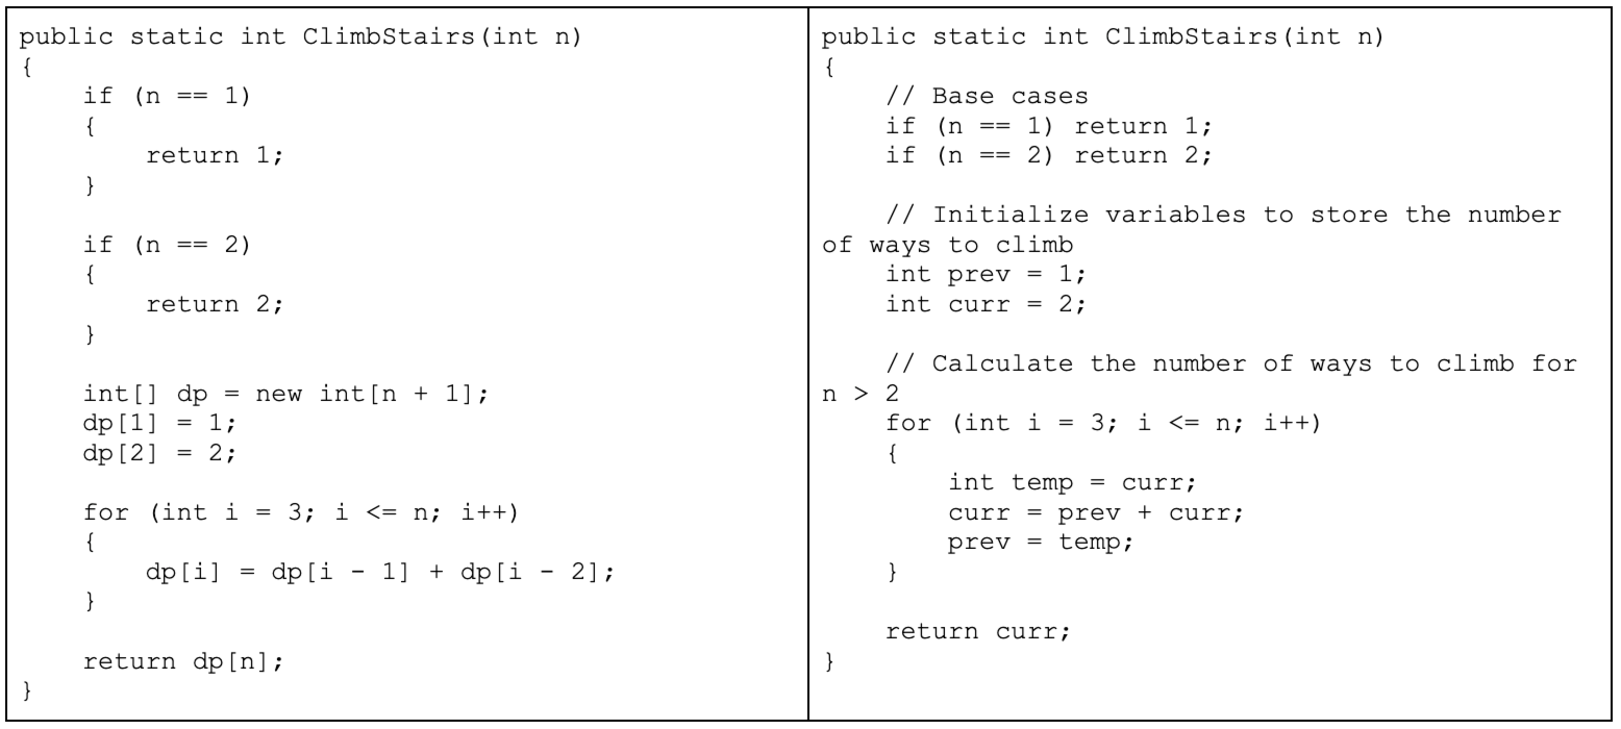
\includegraphics[width=0.75\linewidth]{posttraining/assets/code_system_prompt_example.pdf}
\caption{\label{fig:code_system_prompt_example} \textbf{Improving generated code quality with system prompts.} \emph{Left:} without system prompt \emph{Right:} with system prompt.}
\end{figure}

\textbf{Filtering training data with execution and model-as-judge signals.} 
As described in Section~\ref{subsubsec:data_clean}, we occasionally encounter quality issues in our rejection-sampled data, such as code blocks containing bugs. Detecting these issues in our rejection-sampled data is not as straightforward as it is for our \emph{synthetic code data}, as the rejection-sampled responses typically contain a mix of natural language and code for which the code may not always be expected to be executable. (For example, user prompts may explicitly ask for pseudo-code or edits to only a very small snippet of an executable program.) To address this, we utilize the ``model-as-judge'' approach, where earlier versions of \llamathree assess and assign a binary (0/1) score based on two criteria: code correctness and code style. We retain only those samples that achieve a perfect score of 2. Initially, this stringent filtering led to a regression in downstream benchmark performance, primarily because it disproportionately removed examples with challenging prompts. To counteract this, we strategically revise the responses of some coding data categorized as most challenging until they met the Llama-based ``model-as-judge'' criteria. By refining these challenging problems, the coding data achieves a balance between quality and difficulty, resulting in optimal downstream performance.

\subsubsection{Multilinguality}
\label{subsubsec:multilingual}
We describe how we improve Llama 3's multilingual capabilities, including training an expert specialized on substantially more multilingual data, sourcing and generating high quality multilingual instruction tuning data for German, French, Italian, Portuguese, Hindi, Spanish, and Thai, and tackling specific challenges of multilingual language steering to enhance the overall performance of our model. 

\textbf{Expert training.} Our \llamathree pre-training data mix contains significantly more English tokens than non-English tokens. To collect higher quality human annotations in non-English languages, we train a \textbf{multilingual expert} by branching off the pre-training run and continuing to pre-train on a data mix that  consists of $90$\% multilingual tokens. We then perform post-training on this expert following Section~\ref{sec:finetuning_modeling}. This expert model is then used to collect higher quality annotations in non-English languages until pre-training was fully complete.

\textbf{Multilingual data collection.} Our multilingual SFT data is derived primarily from sources described below. The overall distribution is 2.4\% human annotations, 44.2\% data from other NLP tasks, 18.8\% rejection sampled data, and 34.6\% translated reasoning data.
\begin{itemize}
        \item \textbf{Human annotations}: We collect high-quality, manually annotated data from linguists and native speakers. These annotations mostly consist of open-ended prompts that represent real world use cases. %

        \item \textbf{Data from other NLP tasks}: To further augment, we use multilingual training data from other tasks and rewrite into dialog format. For example, we use data from exams-qa~\citep{hardalov-etal-2020-exams} and Conic10k~\citep{wu2023conic10kchallengingmathproblem}. To improve language alignment, we also use parallel texts from GlobalVoices~\citep{PROKOPIDIS16.778} and Wikimedia~\citep{Tiedemann2012ParallelDT}. We use LID based filtering and Blaser2.0~\citep{seamlessm4t2023} to remove low quality data. For parallel text data, instead of using the bitext pairs directly, we apply a multilingual template inspired by~\citet{weifinetuned} to better simulate real-life conversations in translation and language learning scenarios.
     
        \item \textbf{Rejection sampled data}: We apply rejection sampling on our human annotated prompts to generate high-quality samples for finetuning, with few modifications compared to the process for English data: 
            \begin{itemize} 
                \item \textbf{Generation}: 
                We explored randomly choosing the temperature hyperparameter from the range $0.2-1$ for diverse generations in early rounds of post-training. %
                With high temperature, responses for multilingual prompts can get creative and inspiring, but are also susceptible to unnecessary or unnatural code-switching. In the final round of post-training, we use a constant value of 0.6 to balance the trade-off. Additionally, we used specialized system prompts to improve response format, structure and general readability. 
                \item \textbf{Selection}: Prior to reward model based selection, we implement multilingual-specific checks to ensure high language-match rate between the prompt and response (e.g., a romanized Hindi prompt should not expect a response in Hindi Devanagari script). %
            \end{itemize}
        \item \textbf{Translated data}: We try to avoid using machine-translated data to finetune the model in order to prevent translationese~\citep{bizzoni-etal-2020-human,muennighoff2023crosslingual} or possible name bias~\citep{wang-etal-2022-measuring}, gender bias \citep{10.1162/tacl_a_00401}, or cultural bias~\citep{Ji_Ji_Bouillon_Seligman_2023}. Moreover, we aim to prevent the model from being exposed only to tasks that are rooted in English cultural context, which may not be representative of the linguistic and cultural diversity we aim to capture. We made one exception to this and translated our synthetic quantitative reasoning data (see Section~\ref{subsubsec:reasoning} for details) to improve performance in quantitative reasoning in non-English languages.
        Due to the simple nature of the language in these math problems, the translated samples were found to have little to no quality issues. We observed strong gains on MGSM~\citep{shi2022languagemodelsmultilingualchainofthought} from adding this translated data. 
\end{itemize}

\subsubsection{Math and Reasoning}
\label{subsubsec:reasoning}

We define reasoning as the ability to perform multi-step computations and arrive at the correct final answer. Several challenges guide our approach to training models that excel in mathematical reasoning:

\begin{itemize}
    \item \textbf{Lack of prompts}: As the complexity of questions increases, the number of valid prompts or questions for Supervised Fine-Tuning (SFT) decreases. This scarcity makes it difficult to create diverse and representative training datasets for teaching models various mathematical skills~\citep{yu2023metamath, yue2023mammoth, luo2023wizardmath, mitra2024orca, shao2024deepseekmath,yue2024mammoth2}.
    \item \textbf{Lack of ground truth chain of thought}: Effective reasoning requires a step-by-step solution to facilitate the reasoning process~\citep{wei2022chain}. However, there is often a shortage of ground truth chains of thought, which are essential for guiding the model how to break down the problem step-by-step and reach the final answer \citep{zelikman2022star}.
    \item \textbf{Incorrect intermediate steps}: When using model-generated chains of thought, the intermediate steps may not always be correct~\citep{cobbe2021training,uesato2022solving, lightman2023let, wang2023math}. This inaccuracy can lead to incorrect final answers and needs to be addressed.
    \item \textbf{Teaching models to use external tools}: Enhancing models to utilize external tools, such as code interpreters, allows them to reason by interleaving code and text~\citep{gao2023pal, chen2022program, gou2023tora}. This capability can significantly improve their problem-solving abilities.
    \item \textbf{Discrepancy between training and inference}: There is often a discrepancy between how the model is finetuned during training and how it is used during inference. During inference, the finetuned model may interact with humans or other models, requiring it to improve its reasoning using feedback. Ensuring consistency between training and real-world usage is crucial for maintaining reasoning performance.
\end{itemize}

To address these challenges, we apply the following methodologies:

\begin{itemize}
    \item \textbf{Addressing the lack of prompts:} We source relevant pre-training data from mathematical contexts and converted it into a question-answer format which can then be used for supervised finetuning. Additionally, we identify mathematical skills where the model under-performs and actively sourced prompts from humans to teach models such skills. To facilitate this process, we create a taxonomy of mathematical skills~\citep{didolkar2024metacognitive} and ask humans to provide relevant prompts/questions accordingly.
    \item \textbf{Augmenting training data with step-wise reasoning traces}: We use \llamathree~to generate step-by-step solutions for a set of prompts. For each prompt, the model produces a variable number of generations. These generations are then filtered based on the correct answer~\citep{li2024common}. We also do self-verification where \llamathree~is used to verify whether a particular step-by-step solution is valid for a given question. This process improves the quality of the finetuning data by eliminating instances where the model does not produce valid reasoning traces.
    \item \textbf{Filtering incorrect reasoning traces}:  We train outcome and stepwise reward models~\citep{lightman2023let, wang2023math} to filter training data where the intermediate reasoning steps were incorrect. These reward models are used to eliminate data with invalid step-by-step reasoning, ensuring high-quality data for finetuning. For more challenging prompts, we use Monte Carlo Tree Search (MCTS) with learned step-wise reward models to generate valid reasoning traces, further enhancing the collection of high-quality reasoning data~\citep{xie2024monte}.
    \item \textbf{Interleaving code and text reasoning}:  We prompt \llamathree~to solve reasoning problems through a combination of textual reasoning and associated Python code~\citep{gou2023tora}. Code execution is used as a feedback signal to eliminate cases where the reasoning chain was not valid, ensuring the correctness of the reasoning process.
    \item \textbf{Learning from feedback and mistakes}: To simulate human feedback, we utilize incorrect generations (\emph{i.e.}, generations leading to incorrect reasoning traces) and perform error correction by prompting \llamathree~to yield correct generations~\citep{an2023learning, welleck2022generating, madaan2024self}. The iterative process of using feedback from incorrect attempts and correcting them helps improve the model's ability to reason accurately and learn from its mistakes.
\end{itemize}


\subsubsection{Long Context}
\label{subsubsec:long_context}

During the final pre-training stage, we extend the context length of \llamathree from 8K tokens to 128K tokens (see Section~\ref{section:pretraining_training_recipe} for more details). Similar to pre-training, we find that during finetuning we must carefully tune the recipe to balance short and long-context capabilities.

\textbf{SFT and synthetic data generation.} 
Naively applying our existing SFT recipe with only short-context data resulted in significant regressions in long-context capabilities from pre-training, highlighting the need to incorporate long-context data in our SFT data mix. In practice, however, it is largely impractical to get humans to annotate such examples due to the tedious and time-consuming nature of reading lengthy contexts, so we predominantly rely on synthetic data to fill this gap.
We use earlier versions of \llamathree to generate synthetic data based on the key long-context use-cases: (possibly multi-turn) question-answering, summarization for long documents, and reasoning over code repositories, and describe them in greater detail below.

\begin{itemize}
    \item \textbf{Question answering:} We carefully curate a set of long documents from our pre-training mix. We split these documents into chunks of 8K tokens, and prompted an earlier version of the \llamathree model to generate QA pairs conditional on randomly selected chunks. During training, the whole document is used as context.

    \item \textbf{Summarization:} We applied hierarchical summarization of long-context documents by first summarizing the chunks of 8K input length using our strongest \llamathree 8K context model and then summarizing the summaries. During training we provide the full document and prompt the model to summarize the document while preserving all the important details. We also generate QA pairs based on the summaries of the documents and prompt the model with questions that require global understanding of the whole long document.

    \item \textbf{Long context code reasoning:} We parse Python files to identify \texttt{import} statements and determine their dependencies. From here, we select the most commonly depended-upon files, specifically those referenced by at least five other files. We remove one of these key files from a repository and prompt the model to identify which files depended on the missing file and to generate the necessary missing code.
\end{itemize}

We further categorize these synthetically generated samples based on the sequence length (16K, 32K, 64K and 128K) to enable more fine-grained targeting of input lengths.

Through careful ablations, we observe that mixing $0.1$\% of synthetically generated long-context data with the original short-context data optimizes the performance across both short-context and long-context benchmarks. 

\textbf{DPO.} 
We observe that using only short context training data in DPO did not negatively impact long-context performance as long as the SFT model is high quality in long context tasks. We suspect this is due to the fact that our DPO recipe has fewer optimizer steps than SFT.  Given this finding, we keep the standard short-context recipe for DPO on top of our long-context SFT checkpoints.

\subsubsection{Tool Use}
\label{subsubsec:tool_use}

Teaching LLMs to use tools such as search engines or code interpreters hugely expands the range of tasks they can solve, transforming them from pure chat models into more general assistants~\citep{nakano2021webgpt,thoppilan2022lamdalanguagemodelsdialog,parisi2022talm,gao2023pal,mialon2023augmented,schick2024toolformer}. We train \llamathree~to interact with the following tools:


\begin{itemize}
    \item \textbf{Search engine.} \llamathree~is trained to use Brave Search\footnote{\url{https://brave.com/search/api/}} to answer questions about recent events that go beyond its knowledge cutoff or that require retrieving a particular piece of information from the web.
    \item \textbf{Python interpreter.} \llamathree~can generate and execute code to perform complex computations, read files uploaded by the user and solve tasks based on them such as question answering, summarization, data analysis or visualization. 
    \item \textbf{Mathematical computational engine.} \llamathree~can use the Wolfram Alpha API\footnote{\url{https://products.wolframalpha.com/llm-api/documentation}} to more accurately solve math, science problems, or retrieve accurate information from Wolfram's database. 
\end{itemize}
The resulting model is able to use these tools in a chat setup to solve the user's queries, including in multi-turn dialogs. If a query requires multiple tool calls, the model can write a step-by-step plan, call the tools in sequence, and do reasoning after each tool call. %

We also improve \llamathree's zero-shot tool use capabilities --- given in-context, potentially unseen tool definitions and a user query, we train the model to generate the correct tool call. %

\textbf{Implementation.}
We implement our core tools as Python objects with different methods. Zero-shot tools can be implemented as Python functions with descriptions, documentation (\emph{i.e.}, examples for how to use them), and the model only needs the function's signature and docstring as context to generate the appropriate call. We also convert function definitions and calls to JSON format, e.g., for web API calls. All tool calls are executed by the Python interpreter, that must be enabled in the \llamathree~system prompt. Core tools can be individually enabled or disabled in the system prompt. 

\textbf{Data collection.}
Different from~\citet{schick2024toolformer}, we rely on human annotations and preferences to teach \llamathree~to use tools. There are two main differences with the post-training pipeline generally used in \llamathree:
\begin{itemize}
    \item For tools, dialogs often contain more than a single assistant message (e.g., calling the tool and reasoning about the tool output). Thus, we annotate at the message level to collect granular feedback: annotators provide a preference between two assistant messages with the same context or, if both contain major problems, edit one of the messages. The chosen or edited message is then added to the context and the dialog continues. This provides human feedback for both the assistant's ability of calling the tools and reasoning about the tool outputs. Annotators cannot rank or edit the tool outputs. 
    \item We do not perform rejection sampling, as we did not observe gains in our tool benchmarks.
\end{itemize}

To accelerate the annotation process, we start by bootstrapping basic tool use capabilities by finetuning on synthetically generated data from previous \llamathree~checkpoints. Thus, annotators have fewer edits to perform. In a similar spirit, as \llamathree~gradually improves through its development, we progressively complexify our human annotation protocols: we start by single-turn tool use annotations, before moving to tool use in dialogs, and finally annotating for multi-step tool use and data analysis.


\textbf{Tool datasets.}
To create data for tool usage applications, we leverage the following procedure:
\begin{itemize}
    \item \textbf{Single-step tool use:} We start by few-shot generation of synthetic user prompts which, by construction, require a call to one of our core tools (for example, questions that exceed our knowledge cutoff date).
    Then, still relying on few-shot generation, we generate appropriate tool calls for these prompts, execute them, and add the output to the model's context. Finally, we prompt the model again to generate a final answer to the user's query based on the tool output. We end up with trajectories of the following form: system prompt, user prompt, tool call, tool output, final answer. We also filter around $30\%$ this dataset to remove tool calls that cannot be executed or other formatting issues. 
    
    \item \textbf{Multi-step tool use:} We follow a similar protocol and first generate synthetic data to teach the model basic multi-step tool use capabilities. To do this, we first prompt \llamathree~to generate user prompts that require at least two tool calls, that can be the same or different tools from our core set. Then, conditioned on these prompts, we few-shot prompt \llamathree~to generate a solution consisting of interleaved reasoning steps and tool calls, similar to ReAct~\citep{yao2022react}. See Figure~\ref{fig:multi_step_tool_use} for an example of \llamathree~performing a task involving multi-step tool usage. 
    
    \item \textbf{File uploads:} We annotate for the following filetypes: \textsc{.txt, .docx, .pdf, .pptx, .xlsx, .csv, .tsv, .py, .json, .jsonl, .html, .xml}. Our prompts are based on a provided file, and ask to summarize the contents of the file, find and fix bugs, optimize a piece of code, perform data analysis or visualization. See Figure~\ref{fig:file_upload} for an example of \llamathree~performing a task involving a file upload. 
\end{itemize}

After finetuning on this synthetic data, we gather human annotations in diverse and challenging scenarios including multi-turn interactions, more than three step tool use, and instances where a tool call does not yield a satisfying answer.
We augment our synthetic data with different system prompts to teach the model to use tools only when activated. To train the model to avoid calling tools for simple queries, we also add queries from easy math or question answering datasets~\citep{berant-etal-2013-semantic,koncel2016mawps,joshi-etal-2017-triviaqa,amini2019mathqa} and their responses without tools, but with tools activated in system prompt. 

\begin{figure}[t]
    \centering
    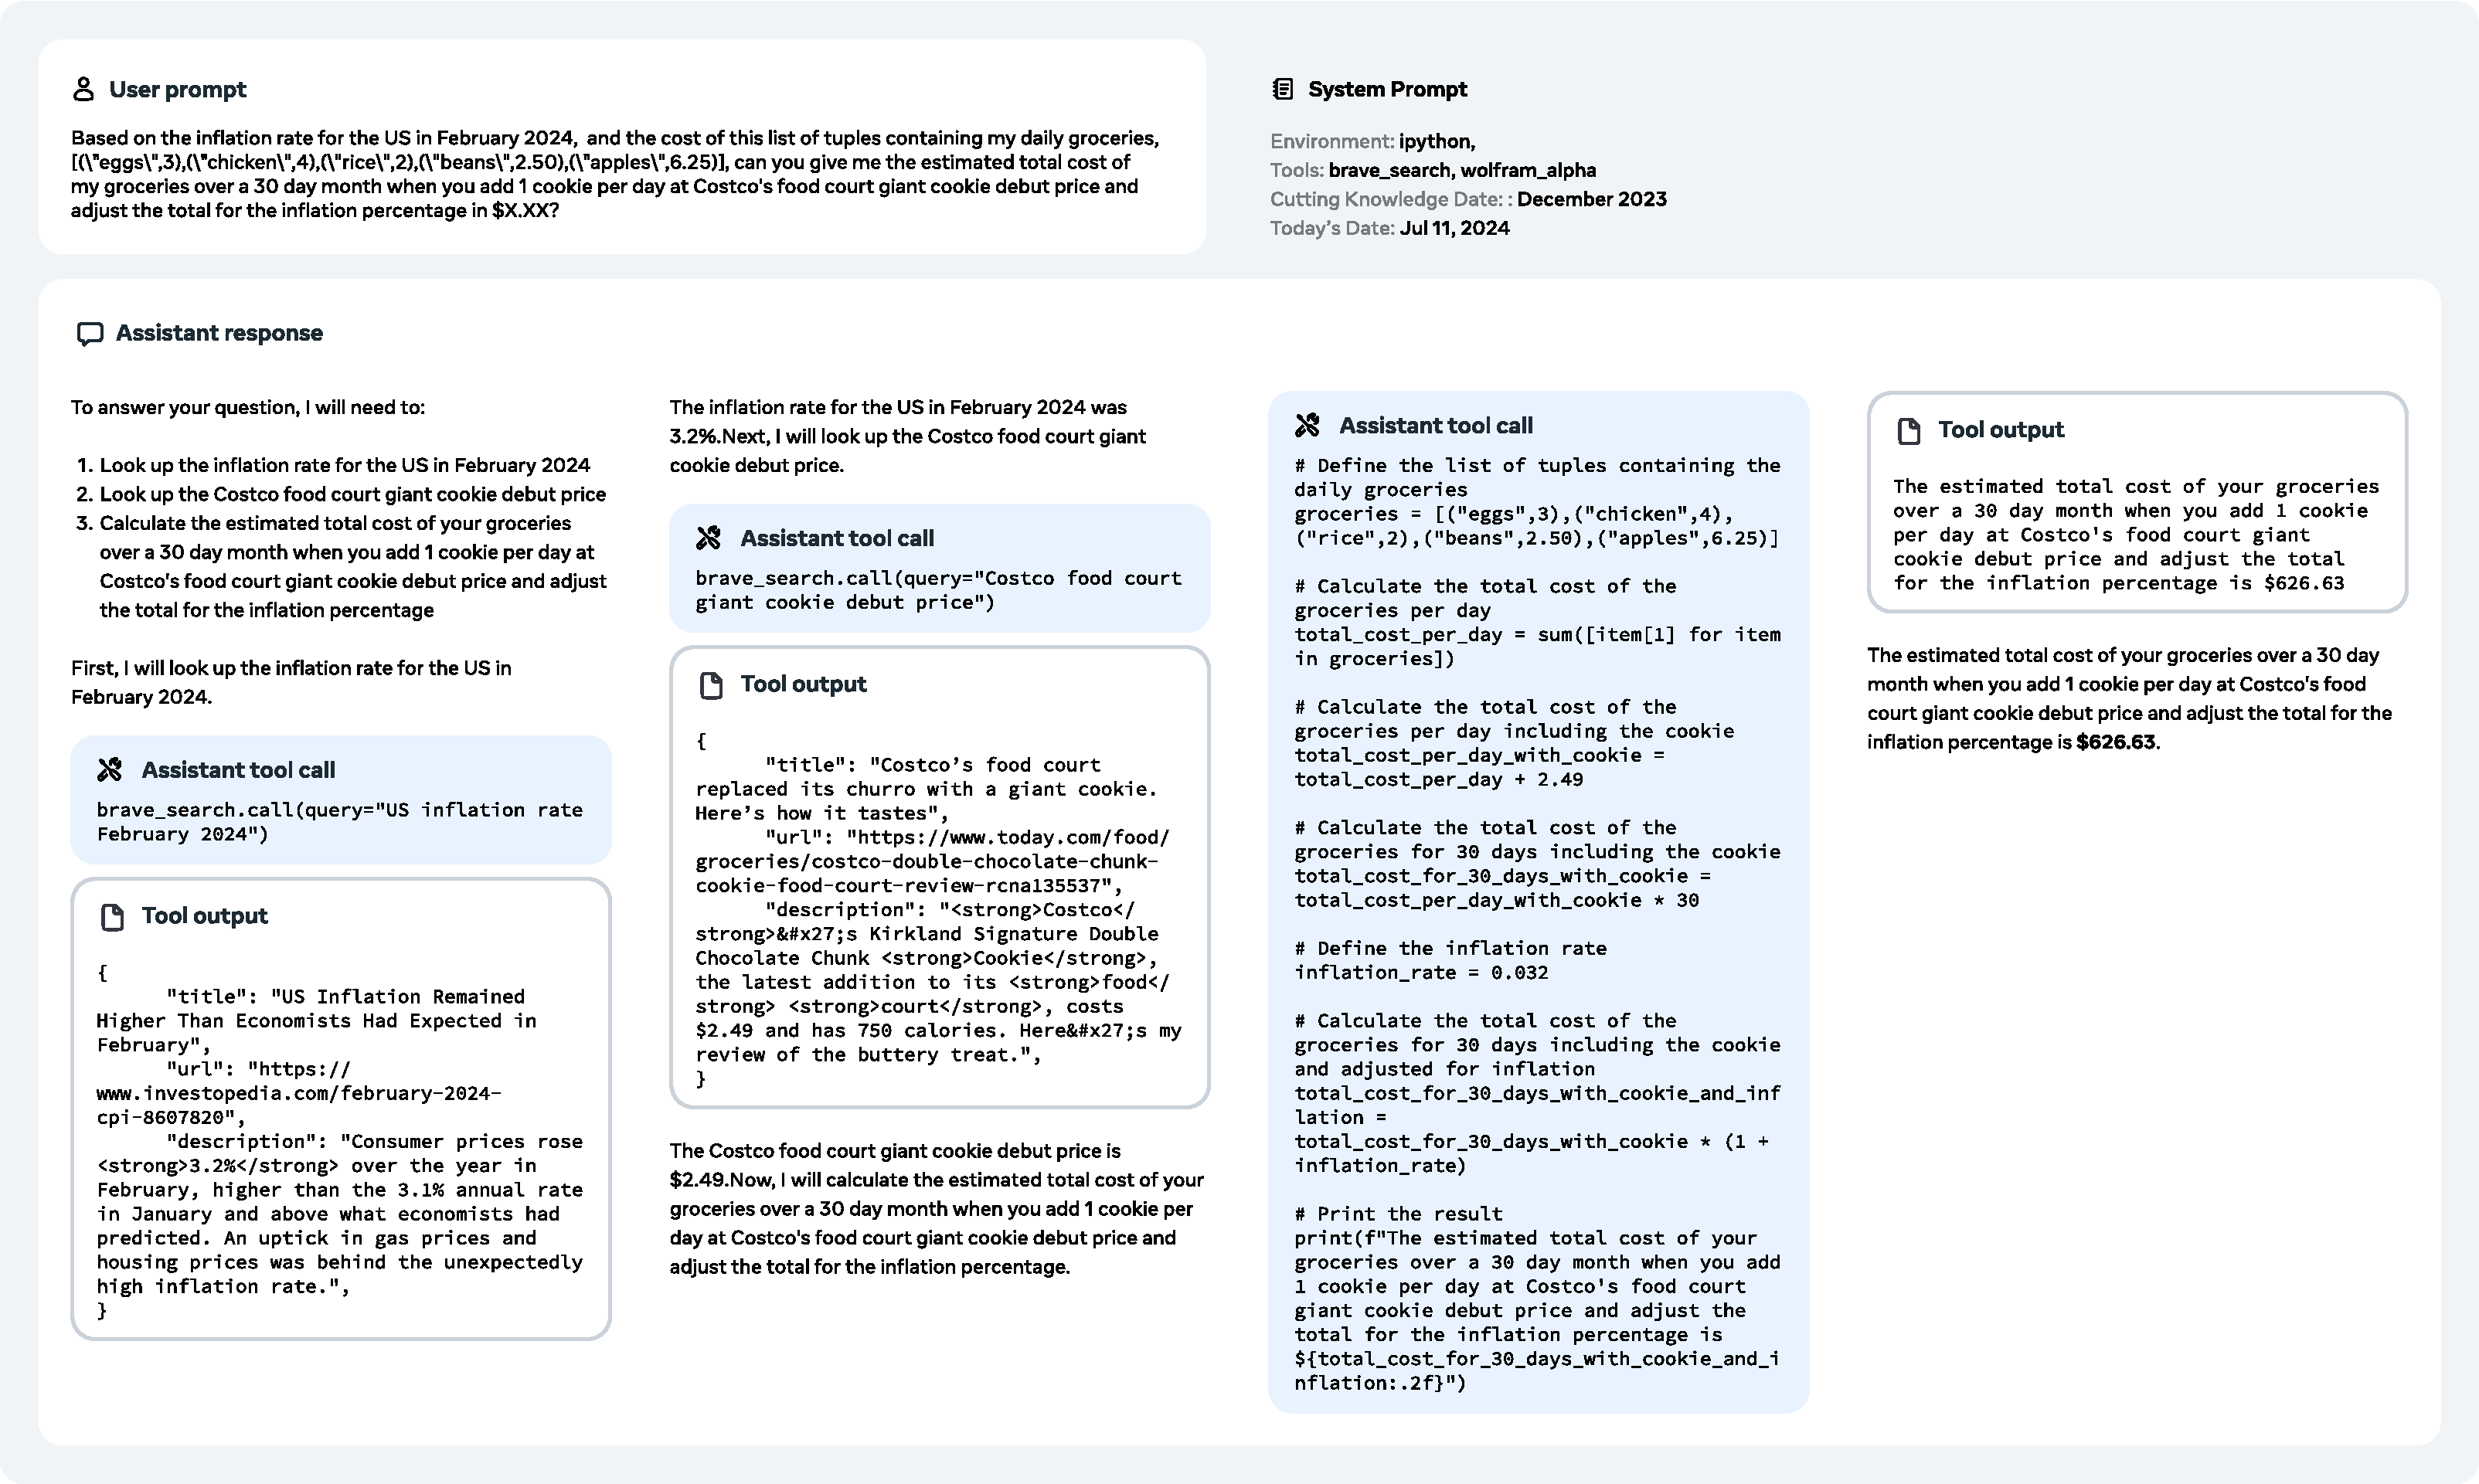
\includegraphics[width=\textwidth]{assets/llama-search-code.pdf}
    \caption{\textbf{Multi-step tool usage.} Example of \llamathree performing multi-step planning, reasoning, and tool calling to solve a task.}
    \label{fig:multi_step_tool_use}
\end{figure}

\textbf{Zero-shot tool use data.}
We improve \llamathree~zero-shot tool use abilities (also referred to as function calling) by finetuning on a large and diverse set of partly synthetic (functions definitions, user query, corresponding call) tuples. We evaluate our model on a set of unseen tools. 
\begin{itemize}
    \item \textbf{Single, nested, and parallel function calling:} %
    Calls can be simple, nested, \textit{i.e.} we pass a function call as an argument of another function, or parallel, \textit{i.e.} the model returns a list of independent function calls. Generating a diverse set of functions, queries and ground truths can be challenging~\citep{mekala2024toolverifier}, and we resort to mining the Stack~\citep{kocetkov2022stack3tbpermissively} to ground our synthetic user queries in real functions. More precisely, we extract function calls and their definitions, clean and filter them, \textit{e.g.} for missing docstrings or non-executable functions, and use \llamathree~to generate a natural language query corresponding to the function call. 

    \item \textbf{Multi-turn function calling:}  We also generate synthetic data for multi-turn dialogs with function calls, following a protocol similar to the one proposed in~\cite{li2023api}. We use multiple agents that generate domains, APIs, user queries, API calls, and responses, while also ensuring that the generated data covers a set of diverse domains and realistic APIs. All agents are variants of \llamathree~prompted in different ways depending on their roles and collaborate in a step-by-step manner. %
    

\begin{figure}[t]
    \centering
    \includegraphics[width=\textwidth]{assets/llama-file-upload-6x.png}
    \caption{\textbf{Processing file uploads.} Example of \llamathree performing analysis and visualization of an uploaded file.}
    \label{fig:file_upload}
\end{figure}

\end{itemize}

\subsubsection{Factuality}\label{subsubsec:factuality}

Hallucinations remain a major challenge for large language models. Models tend to be overconfident, even in domains where they have little knowledge. Despite these shortcomings, they are often used as knowledge bases, which can lead to risky outcomes such as the spread of misinformation. While we recognize that factuality can go beyond hallucinations, we took a hallucination-first approach here.


We follow the principle that post-training should align the model to ``know what it knows'' rather than add knowledge~\citep{gekhman2024does,mielke2020metacognition}. Our primary approach involves generating data that aligns model generations with subsets of factual data present in the pre-training data. To achieve this, we develop a knowledge probing technique that takes advantage of \llamathree's in-context abilities. This data generation process involves the following procedure:

\begin{enumerate}
    \item \textbf{Extract a data snippet} from the pre-training data. %
    \item \textbf{Generate a factual question} about these snippets (context) by prompting \llamathree.
    \item \textbf{Sample responses} from \llamathree~to the question.
    \item \textbf{Score the correctness} of the generations using the original context as a reference and \llamathree~as a judge.
    \item \textbf{Score the informativeness} of the generations using \llamathree~as a judge.
    \item \textbf{Generate a refusal} for responses which are consistently informative and incorrect across the generations, using \llamathree.
\end{enumerate}

We use data generated from the knowledge probe to encourage the model to only answer questions which it has knowledge about, and refuse answering those questions that it is unsure about. %
Further, pre-training data is not always factually consistent or correct. We therefore also collect a limited set of labeled factuality data that deals with sensitive topics where factually contradictory or incorrect statements are prevalent. %

\subsubsection{Steerability}
\label{subsubsec:steerability}

Steerability is the ability to direct the model's actions and outcomes to meet developer and user specifications. As \llamathree is a generic foundational model, it should be maximally steerable to different downstream use cases easily. For \llamathree, we focus on enhancing its steerability through system prompt with natural language instructions, especially around response length, format, tone and character/persona. 

\textbf{Data collection.}  We collect steerability preference samples within the general English category by asking annotators to design different system prompts for \llamathree. Annotators then engage in conversations with the models to evaluate their consistency in following instructions defined in system prompts over the course of the conversation. We show an example customized system prompt used for enhancing steerability below:


\begin{tcolorbox}
\texttt{You are a helpful and cheerful AI Chatbot that acts as a meal plan assistant for busy families. The family consists of 2 adults, 3 teenagers, and 2 preschoolers. Plan two or three days at a time and use leftovers or extra ingredients for the second day's plan. The user will let you know if they want two or three days. If they don't, assume three days. Each plan should include breakfast, lunch, snack, and dinner. Ask the user if they approve of the plan or need adjustments. After they approve provide a grocery list with family size in mind. Always keep family preferences in mind and if there's something that they don't like provide a substitution. If the user is not feeling inspired then ask them what's the one place they wish they could visit on vacation this week and then suggest meals based on that location's culture. Weekend meals can be more complex. Weekday meals should be quick and easy. For breakfast and lunch, easy food like cereal, English muffins with pre-cooked bacon, and other quick easy foods are preferred. The family is busy. Be sure to ask if they have essentials and favorites on hand like coffee or energy drinks so they don't forget to buy it. Remember to be budget-conscious unless it's a special occasion.}
\end{tcolorbox}

\textbf{Modeling.} After we collect the preference data, we leverage this data in reward modeling, rejection sampling, SFT, and DPO to enhance \llamathree's steerability. 
